%!TEX root=ClockPendulumAnalyzer.tex
\section{Raspberry Pi}
\begin{frame}
%image with all the technologies
\end{frame}

\subsection{Aufbau - Architektur}
\begin{frame}
    \frametitle{Aufbau - Architektur}
    \begin{columns}[c] % the "c" option specifies center vertical alignment
        \column{.5\textwidth}
        \begin{itemize}
            \item<1->3-Layer Architektur
            \item<1->mögliche 2-Tier Verteilung
            \item<1->Daten-Transfer-Objekt und REST
        \end{itemize}
        \column{.5\textwidth} % column designated by a command
        \begin{figure}
            \centering
            \begin{overprint}
                \onslide<1>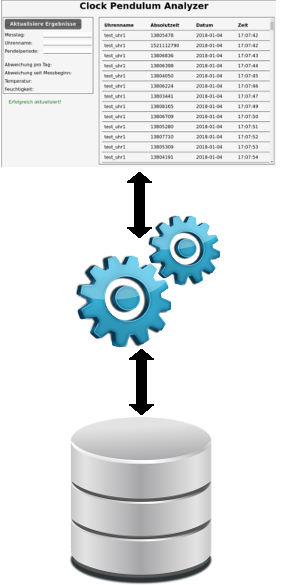
\includegraphics[width=.5\textwidth]{3layer.png}
                \onslide<2->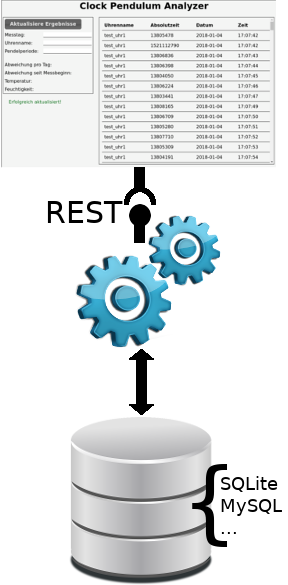
\includegraphics[width=.5\textwidth]{3layer_rest.png}
            \end{overprint}
        \end{figure}
    \end{columns}
\end{frame}

\subsection{Technologien}
\begin{frame}

\end{frame}

\subsection{C++ Software}
\begin{frame}

\end{frame}

\subsection{Schnittstellen}
\begin{frame}

\end{frame}